\documentclass{article}
\usepackage{amsmath}
\usepackage{amssymb}
\usepackage{bm}
\usepackage{graphicx}
\usepackage{epstopdf}
\DeclareGraphicsRule{.tif}{png}{.png}{`convert #1 `basename #1 .tif`.png}
\usepackage{color}
\pagestyle{plain}
%\pagestyle{empty}
\textheight 9 true in
\textwidth 6.5 true in
\hoffset -.75 true in
\voffset -.75 true in
 
\mathsurround=2pt  \parskip=2pt
\def\crv{\cr\noalign{\vskip7pt}} 
\def\a{\alpha } \def\b{\beta } \def\d{\delta } \def\D{\Delta } \def\e{\epsilon }
\def\g{\gamma } \def\G{\Gamma} \def\k{\kappa} \def\l{\lambda } \def\L{\Lambda }
\def\th{\theta } \def\Th{\Theta} \def\r{\rho} \def\o{\omega} \def\O{\Omega}
\def\ve{\varepsilon} 

\def\sA{{\cal A}} \def\sB{{\cal B}} \def\sC{{\cal C}} \def\sI{{\cal I}}
\def\sR{{\cal R}} \def\sF{{\cal F}} \def\sG{{\cal G}} \def\sM{{\cal M}}
\def\sT{{\cal T}} \def\sH{{\cal H}} \def\sD{{\cal D}} \def\sW{{\cal W}}
\def\sL{{\cal L}} \def\sP{{\cal P}} \def\s{\sigma } \def\S{\Sigma}
\def\sU{{\cal U}} \def\sV{{\cal V}} \def\sY{{\cal Y}}

\def\gm{\gamma -1}
\def\summ{\sum_{j=1}^4}

\def\bb{{\bm b}} \def\yb{{\bm y}}
\def\ub{{\bm u}}  \def\xb{{\bm x}} \def\vb{{\bm v}} \def\wb{{\bm w}}
\def\omegab{{\bm \omega}} \def\rb{{\bm r}} \def\ib{{\bm i}} \def\jb{{\bm j}}
\def\lb{{\bm l}} \def\kb{{\bm k}} \def\Ab{{\bm A}} \def\fb{{\bm f}} \def\Ub{{\bm U}}
\def\Fb{{\bm F}} \def\nb{{\bm n}} \def\Db{{\bm D}} \def\eb{{\bm e}}
\def\gb{{\bm g}}  \def\Gb{{\bm G}} \def\hb{{\bm h}} \def\Yb{{\bm Y}} \def\Rb{{\bm R}} 
\def\Tb{{\bm T}}

\def\As1{{\bf {\cal A}}_1}\def\DO{{\cal D}_0} \def\UO{{\cal U}_0}
\def\ie{{\it{i.e.}}}

\def\ubbar{{\bf {\bar{u}}}} \def\sbar{{\bar{\sigma }}} \def\ubar{{\bar{u}}}  
\def\abar{{\bar{a}}} \def\vbar{{\bar{v}}}  \def\rbar{{\bar{\rho}}}
\def\pbar{{\bar{p}}} \def\ebar{{\bar{e}}} \def\Tbar{{\bar{T}}}
\def\bbar{{\bar{\beta}}} \def\Mbar{{\bar{M}}}  \def \sMbar{{\bar{\cal M}}}
\def\Ebar{{\bar{E}}} \def\sMbar{{\bar{\cal M}}}
\def\sPbar{{\bar{\cal P}}} \def\xbar{{\bar{x}}}

\newcommand{\pdv}[2]{\frac{\partial#1}{\partial#2}}
\newcommand{\dv}[2]{\frac{d#1}{d#2}}
\newcommand{\ord}[2]{#1^{(#2)}}
\newcommand{\vct}[1]{\vec{#1}}

 \newcommand{\bc}{\begin{center}}
 \newcommand{\ec}{\end{center}}
 
 \newcommand{\bq}{\begin{equation}}
 \newcommand{\eq}{\end{equation}}
 
 \newcommand{\beqs}{\begin{eqnarray}}
 \newcommand{\eeqs}{\end{eqnarray}}
 
 \newcommand{\beqa}{\begin{eqnarray*}}
 \newcommand{\eeqa}{\end{eqnarray*}}
 
 \newcommand{\ol}{\overline}
 \newcommand{\ul}{\underline}
 
 \newcommand{\dint}{{\int \!\! \int \!\!}}
 \newcommand{\tint}{{\int \!\! \int \!\! \int \!\!}}
 
 \newcommand{\bfig}{\begin{figure}}
 \newcommand{\efig}{\end{figure}}
 
 \newcommand{\cen}{\centering}
 \newcommand{\n}{\noindent}
 
 \newcommand{\btab}{\begin{table}}
 \newcommand{\etab}{\end{table}}
 
 \newcommand{\btbl}{\begin{tabular}}
 \newcommand{\etbl}{\end{tabular}}
 
 \newcommand{\bdes}{\begin{description}}
 \newcommand{\edes}{\end{description}}
 
 \newcommand{\benum}{\begin{enumerate}}
 \newcommand{\eenum}{\end{enumerate}}
 
 \newcommand{\bite}{\begin{itemize}}
 \newcommand{\eite}{\end{itemize}}
 
 \newcommand{\cle}{\clearpage}
 \newcommand{\npg}{\newpage}
 
 \newcommand{\bss}{\begin{singlespace}}
 \newcommand{\ess}{\end{singlespace}}
 
 \newcommand{\bhalf}{\begin{onehalfspace}}
 \newcommand{\ehalf}{\end{onehalfspace}}
 
 \newcommand{\bds}{\begin{doublespace}}
 \newcommand{\eds}{\end{doublespace}}
 
 \newcommand{\eps}{\mbox{$\epsilon$}} 
 \newcommand{\stilde}{\mbox{$\tilde s$}} 
 \newcommand{\shat}{\mbox{$\hat s$}} 

 \newcommand{\blue}{\color{blue}}
 \newcommand{\red}{\color{red}}
 \newcommand{\magenta}{\color{magenta}}
 \newcommand{\green}{\color{green}}
 \newcommand{\nc}{\normalcolor}




%\pagestyle{empty}
\begin{document}

\begin{center}
\large{ MATH-6620 \hspace{1in}  PERTURBATION METHODS \hspace{1in}SPRING 2016\\ Homework-3 \\ Assigned Wednesday February 24, 2016 \\ Due Monday March 7, 2016}\end{center}




\bc {\bf PROBLEMS} \ec

\benum


% Problem 1
\item Consider the initial-value problem
\begin{equation*}
\e \frac{dy}{dt} = ty, \quad y(-1) = 1.
\end{equation*}
\benum
\item Find the exact solution and discuss its qualitative character.  Plot it on the interval $t \in [-1,1]$ for $\e = 0.25.$
Construct a leading-order asymptotic solution for $\e>0$ and small, and discuss whether it is able to capture all significant features of the exact solution.
\item Repeat part (a) for the slightly altered differential equation
\begin{equation*}
\e \frac{dy}{dt} = ty+\e, \quad y(-1) = 1.
\end{equation*}
Discuss what you find.  Any surprises?
\eenum

Solution:\\

\benum
\item $$\e \frac{dy}{dt} = ty, \quad y(-1) = 1$$
 is a separable equation with exact solution:
 $$y=e^{(t^2-1)/2\e}.$$
 The graph of this solution with $\e=0.25$ is included here.
\begin{figure}[h]
  \centering
  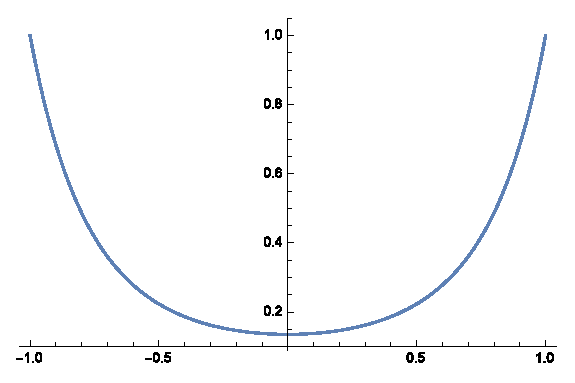
\includegraphics[width=3in]{ass3no1prta}
  \caption{Mathematica Plot of $exp[2(t^2-1)]$}
\end{figure}
To construct a leading-order asymptotic solution for $0<\e<<1$, we let $y(t;\e)\sim y_0(t;\e)$ and let $\e\to 0$ to get
$$0=ty_0\implies y_0=0.$$
As $y_0=0$ does not satisfy the initial condition we suppose that there is a boundary layer of thickness $\delta$ at $t=-1$. Thus we let $t=\delta \tau -1$ and $y(t;\e)=Y(\tau;\e)$. This gives the differential equation
$$\frac{\e}{\delta}Y'=(\delta\tau-1)Y,\quad Y(0;\e)=1.$$
We can determine that $\delta=\e$ by balancing the $\e/\delta$ and the $O(1)$ term. Thus we have
$$Y'=(\e\tau-1)Y,\quad Y(0;\e)=1.$$
If we let $Y(\tau;\e)\sim Y_0(\tau,\e)$ and collect only the $O(1)$ terms we get the differential equation governing the leading order asymptotic solution in the inner layer:
$$Y_0'=-Y_0,\quad Y_0(0)=1$$
with solution
$$Y_0=e^{-\tau}.$$
We now perform Van Dyke matching of the inner and outer approximations to get
$$y_0(t;\e)=0,\quad Y_0(\tau;\e)=e^{-\tau}\implies Y_0(t;\e)=e^{-(t+1)/\e}$$
As $\e\to0$, $Y_0(t;\e)\to 0.$ Thus the composite leading-order asymptotic expansion is
$$y_c(t;\e)=e^{-(t+1)/\e}.$$
The graph of this solution with $\e=0.25$ is included here.
\begin{figure}[h]
\centering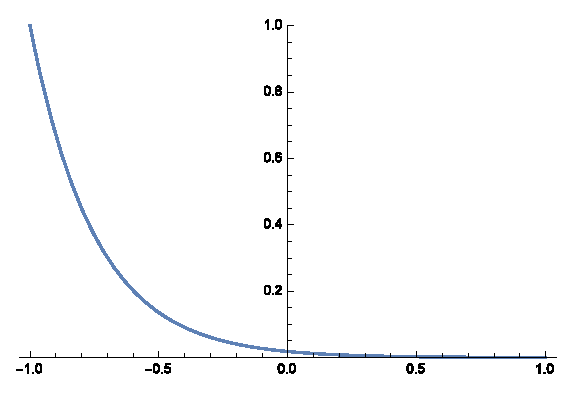
\includegraphics[width=3in]{ass3no1prta2}
\caption{Mathematica Plot of $exp[-4(t+1)]$}
\end{figure}
Overlaying the previous two plots (pictured at the top of the proceeding page) gives a clear indication of which features are captured within the leading-order asymptotic expansion as compared to the exact solution.
\begin{figure}[t]
\centering
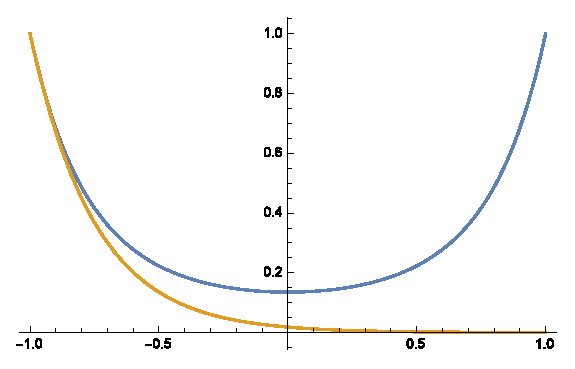
\includegraphics[width=3in]{ass3no1prta3}
\caption{Mathematica Plot of $exp[-4(t+1)]$ and $exp[2(t^2-1)]$}
\end{figure}
The graph shows that we capture the initial value and the initial decay of the function at that point with both the asymptotic and the exact solutions. However, the asymptotic expansion does not show the symmetry or the growth evident in the exact solution.
\pagebreak

\item
$$\e \frac{dy}{dt} = ty+\e, \quad y(-1) = 1$$
has exact solution
$$y(t;\e)=\frac{1}{2}e^{(t^2-1)/2\e}\left(2+e^{1/2\e}\sqrt{2\e\pi}erf\left(\frac{1}{\sqrt{2\e}}\right)+e^{1/2\e}\sqrt{2\e\pi}erf\left(\frac{t}{\sqrt{2\e}}\right)\right).$$
The plot of this solution over the domain in question is included here:
\begin{figure}[h]
\centering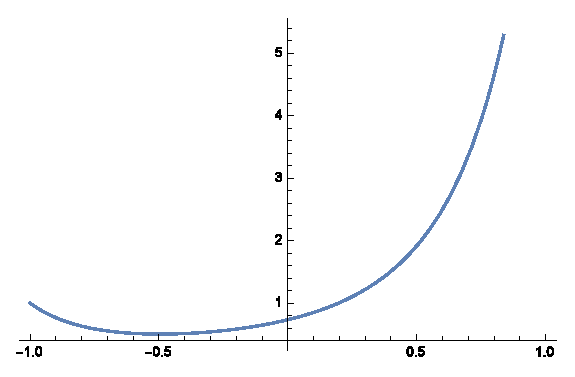
\includegraphics[width=3in]{ass3no1prtb}
\caption{Mathematica Plot of exact solution}
\end{figure}
However, if we find the leading-order asymptotic expansion, we will find the same expansion as before. If we let $y(t;\e)\sim y_0(t;\e)$ and $\e\to 0$ we get the equation
$$0=t y_0\implies y_0=0.$$
As this approximation does not satisfy the boundary condition, we let $t=\delta\tau-1$ and $y(t;\e)=Y(\tau;\e).$ We then get the differential equation
$$\frac{\e}{\delta}Y'=(\delta \tau-1)Y+\e,\quad Y(0)=1.$$
Dominant balance requires $\delta=\e$ giving the equation
$$Y'=(\e\tau-1)Y+\e,\quad Y(0)=1.$$
If we let $Y(\tau;\e)\sim Y_0(\tau;\e)$ and collect the $O(1)$ terms we get the same differential equation for the inner solution as did in part (a):
$$Y_0'=-Y_0,\quad Y_0(0)=1.$$
Hence we have the same asymptotic expansion as before
$$y_c=e^{-(t+1)/\e},$$
with plot included in the previous part of the solution. Plotting both solutions on the same graph shows the distinctions between the asymptotic expansion and the exact solution.
\begin{figure}
\centering
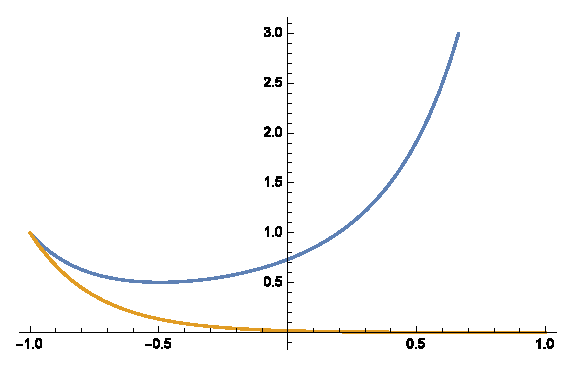
\includegraphics[width=3in]{ass3no1prtb2}
\caption{Mathematica Plot of $y_c$ and $y$}
\end{figure}
The graph shows that the leading-order asymptotic expansion only captures a very small part of the exact solution; namely the initial condition and some initial decay. The asymptotic solution fails to capture the eventual exponential growth and the parabolic smoothness of the exact solution.
\eenum


% Problem 2
\item
Consider the initial-value problem
\begin{equation*}\
e \frac{dy}{dt} +ty = t e^{-t}, \quad y(0) = 2.
\end{equation*}
For $\e >0$ and small, find the leading-order composite solution.\\

Solution:\\

We begin by assuming $y(t;\e)\sim y_0(t;\e)$ and collect the leading-order terms of the resulting differential equation and get
$$y_0=e^{-t}.$$
As $y_0(0)=1\neq 2$ we know that we have an initial layer at $t=0$. Thus we let $t=\delta \tau$ and $y(t;\e)=Y(\tau;\e)$. We then get the differential equation
$$\frac{\e}{\delta}Y'+\delta\tau Y=\delta\tau e^{-\delta \tau},\quad Y(0)=2.$$
Dominant balance requires $\e/\delta=\delta\implies \delta=\sqrt{\e}$, resulting in the differential equation
$$Y'+\tau Y=\tau e^{-\sqrt{\e}\tau},\quad Y(0)=2.$$
If we let $Y(\tau;\e)\sim Y_0(\tau;\e)$, expand the exponential term and collect the resulting order one terms to get the differential equation for the leading order inner solution
$$Y_0'+\tau Y_0=\tau,\quad Y_0(0)=2.$$
This equation can be solved by the method of integrating factors to give
$$Y_0=1+e^{-\tau^2/2}.$$
We now perform Van Dyke matching to see if the inner and outer solutions match and can be combined to produce a reasonable composite solution. We begin by expressing the outer solution in the inner variable and the inner solution in the outer variable.
$$y_0(\tau;\e)=e^{-\sqrt{\e}\tau},\;\text{ and }\;Y_0(t;\e)=1+e^{-t^2/2\e}.$$
Then if we take the limit as $\e\to 0$ of each, we find that
$$y_0\sim 1\;\text{ and }\; Y_0\sim 1.$$
Then we can form a composite expansion $y_c=y_0+Y_0-1$ to get the leading-order composite solution
$$y_c=e^{-t}+e^{-t^2/2\e}.$$


% Problem 3
\item Consider the initial-value problem for the system of equations
\begin{eqnarray*}
\frac{dx}{dt} &=& xy, \\
\e \frac{dy}{dt} &=& y-y^3,
\end{eqnarray*}
with initial conditions
\begin{equation*}
x(0) = \a, \;\; y(0) = \b.
\end{equation*}
\benum
\item For $\e>0$ and small, seek an outer solution of the form $x(t;\e) \sim x_0(t), \; y(t;\e) \sim y_0(t).$  Consider all possibilities, and note that the initial conditions will not be met, in general.

\item Consider an initial layer by using the stretching $t = \d(\e) \tau,\;\; x(t;\e) = X(\tau;\e), \; y(t;\e) = Y(\tau;\e),$ where $\d$ is to be found by a suitable argument.  Seek an inner solution of the form $X(\tau;\e) \sim X_0(\tau), \; Y(t;\e) \sim Y_0(\tau).$  Construct the inner solution for (i) $\b >0,$ (ii) $\b < 0$ and (iii) $\b = 0.$  For each case determine the leading-order composite solution.
\eenum

Solution:\\
\benum
\item The outer solutions of the differential equations boil down to three cases. We first let $x(t;\e)\sim x_0(t)$ and $y(t;\e)\sim y_0(t)$ then we collect the $O(1)$ terms to get the system of equations
    $$\left\{\begin{array}{c}x_0'=x_0y_0\\0=y_0-y_0^3\end{array}\right..$$
    It is clear to see that the second equation in the system has 3 solutions, $y_0=-1,0,1$ and that each choice of solution gives a different solution for $x_0$.
    \benum
    \item We first let $y_0=-1$, then the first equation in the above system becomes
    $$x_0'=-x_0 $$
    with solution
    $$x_0=Ae^{-t}.$$
    If we wish to satisfy the initial conditions, $\beta=-1$ and $A=0\implies x_0=0$, giving the solution $y_0=-1$ and $x_0=0$.
    \item Now we let $y_0=0$, then the first equation in the system in question becomes
    $$x_0'=0\implies x_0=B.$$
    If we wish to satisfy the initial conditions here, $\beta=0$ and $B=0\implies x_0=0$, giving the trivial solution $y_0=x_0=0.$
    \item Third, we let $y_0=1.$ The first equation in the first-order asymptotic system then becomes
    $$x_0'=x_0\implies x_0=Ce^t.$$
    Satisfying the boundary conditions gives $x_0=0,\quad\beta=1$.
    \eenum

\item We find the inner solution by first determining the correct scaling on the independent variable. We let $\tau=\frac{t}{\delta}$, and define $x(t;\e)=X(\tau;\e)$ and $y(t;\e)=Y(\tau;\e).$ Then the system of differential equations becomes
    $$\left\{\begin{array}{cc}\frac{1}{\delta}\frac{dX}{d\tau}=XY,&X(0)=0\\\frac{\e}{\delta}\frac{dY}{d\tau}=Y-Y^3,&Y(0)=\beta\end{array}\right..$$
    Dominant balance dictates then that $\delta=\e.$ If we then let $X(\tau;\e)\sim X_0(\tau)$ and $Y(\tau;\e)=Y_0(\tau)$ and collect the resulting $O(1)$ terms, we get the system
    $$\left\{\begin{array}{cc}\frac{dX_0}{d\tau}=0,&X_0(0)=0\\ \frac{dY_0}{d\tau}=Y_0-Y_0^3,&Y_0(0)=\beta\end{array}\right..$$
    This system has the solution
    $$\begin{array}{c}X_0(\tau)=0\\Y_0(\tau)=\frac{\beta e^{\tau}}{\sqrt{\beta^2e^{2\tau}+1-\beta^2}}\end{array}.$$
    Clearly this solution holds for any value of $\beta.$ We will now form the composite solutions.
    \benum
    \item First we look at $\beta>0,$ specifically $\beta=1.$ Here $X_0(\tau)=0$, $Y_0(\tau)=1,$ which is exactly the same as $x_0(t)=Ce^t$, $y_0(t)=1$ when $C=0.$ Thus the composite solution for this case is
        $$x_c(t)=0,\quad y_c(t)=1.$$
    \item Now we form the composite solution for $\beta>0$, $\beta\neq 1.$ Here we must use Van Dyke matching. The outer solution is of the same form as before, $x_0(t)=Ce^t$, $y_0(t)=1,$ which when written in the inner variable becomes $x_0(\tau)=Ce^{\e\tau}$, $y_0(\tau)=1.$ The inner solution in this case, written in the outer variable becomes $X_0(t)=0,$ and
        $$Y_0(t)=\frac{\beta e^{t/\e}}{\sqrt{\beta^2e^{2t/\e}+1-\beta^2}}.$$
        If we take the limit of each outer solution and inner solution as $\e\to0 $, we find
        $$x_0\to C,\quad X_0\to 0,$$
        $$y_0\to1,\quad Y_0\to 1.$$
        Therefore we know $C=0$ and we form the composite solution in this case
        $$x_c=0,\quad y_c=\frac{\beta e^{t/\e}}{\sqrt{\beta^2e^{2t/\e}+1-\beta^2}}.$$
    \item Now we switch to looking at $\beta<0.$ First we investigate the case where $\beta=-1.$ Here $Y_0=-1$ and $y_0=-1.$ Similarly, $X_0=0$ while $x_0=Ae^{-t}$. For the inner and outer $X$ solutions to match, $A=0$. Thus the composite solution in this case is
        $$x_c=0,\quad y_c=-1.$$
    \item Here we consider all other negative $\beta$ with $\beta<0$, $\beta\neq-1$. Again we use Van Dyke matching. We first express the inner solution in the outer variable and the outer solution in the inner variable.
        $$X_0(t)=0,\quad Y_0(t)=\frac{\beta e^{t/\e}}{\sqrt{\beta^2e^{2t/\e}+1-\beta^2}},$$
        $$x_0(\tau)=Ae^{\e\tau},\quad y_0(\tau)=-1.$$
        Then taking the limit as $\e\to 0$ we find
        $$X_0\sim 0,\quad Y_0\sim -1,$$
        and
        $$x_0\sim A,\quad y_0\sim -1.$$
        Thus matching requires $A=0$ and we get the composite solution
        $$x_c(t)=0,\quad y_c(t)= \frac{\beta e^{t/\e}}{\sqrt{\beta^2e^{2t/\e}+1-\beta^2}}.$$
    \item Lastly we look at the case where $\beta=0.$ The outer solution here is $x_0(t)=B$, $y_0(t)=0.$ The Inner solution here is simply the trivial solution $X_0(\tau)=0,$ $Y_0(\tau)=0.$ Thus matching simply tells us that $B=0.$ Then the composite solution is the trivial solution
        $$x_c(t)=0,\quad y_c(t)=0.$$
        \eenum
        \eenum





\item Consider the problem
\begin{equation*}
(x^2+\e y)y' + 2xy = \frac{3\e}{2y}, \quad y(1;\e) = 1.
\end{equation*}
Of interest is the domain $0\le x \le 1.$  Find the first two terms of an outer expansion, for $\e>0$ and small, satisfying the boundary condition at $x=1.$  Show that this expansion is not uniformly valid as $x \to 0.$  Find the breakdown, rescale and hence find the first term of the inner expansion valid near $x=0.$  Find the dominant asymptotic behavior of $y$ as $x \to 0.$\\

Solution:\\

We begin by finding the leading order outer asymptotic expansion by letting $y(x;\e)\sim y_0(x;\e)$ and collect only the $O(1)$ terms, resulting in the equation
$$2xy_0(xy_0'+2y_0)=0,\quad y_0(1)=1.$$
Since the trivial solution $y_0=0$ does not satisfy the boundary condition, we use the method of integrating factor to solve for $y_0$ and we get
$$y_0(x)=\frac{1}{x^2}.$$
We can then find the second term of the outer expansion by letting $y(x;\e)\sim y_0(x;\e)+\e y_1(x;\e)$ and collecting the $0(\e)$ terms. This gives
$$y_1'+\frac{2}{x}y_1=\frac{3}{2}+2x^{-7},\quad y_1(1)=0.$$
Solving with the method of integrating factor results in
$$y_1=\frac{1}{2}\left(x-\frac{1}{x^6}\right).$$
Thus the two term outer expansion is
$$y\sim \frac{1}{x^2}+\frac{\e}{2}\left(x-\frac{1}{x^6}\right).$$
Clearly the expansion breaks down when
$$\frac{1}{x^2}=\frac{\e}{x^6}\implies x=O(\e^{1/4}).$$
If we simply let $\e^{1/4}\xi=x$ and $y(x;\e)=Y(\xi;\e)$, we will be unable to determine the constant that arises in solving for the leading order inner solution, and we will still be left with a singularity at $x=0$. Thus we scale $x$ in the way listed above, but we also scale $\delta y(x;\e)=Y(\xi;\e).$ This results in the ODE
$$\left(\e^{1/2}\xi^2+\frac{\e}{\delta}Y\right)\frac{1}{\e^{1/4}\delta}Y'+\frac{2\e^{1/4}\xi}{\delta}Y=\frac{3\e\delta}{2 Y}.$$
Dominant balance dictates that we must balance the first three terms, and thus we require $\delta=\e^{1/2}$. If we let $Y(\xi;\e)\sim Y_0(\xi;\e)$ and collect the resulting $O(1)$ terms we get the Bernoulli equation
$$(\xi^2+Y_0)Y_0'+2\xi Y_0=0,$$
with solution
$$Y_0 =-\xi^2+\sqrt{C+\xi^4}.$$
Note we choose the positive solution here to balance the quadratic terms as $\xi\to \infty$. The constant $C$ may be chosen from data, as we only know that
$$Y_0(0)=\sqrt{C}.$$
If we rewrite the inner solution in the outer variable and the outer solution in the inner variable, we get
$$y_0(\xi)+\e y_1(\xi)=\frac{1}{\sqrt\e\xi^2}+\frac{\e^{5/4}\xi}{2}-\frac{1}{\sqrt{\e}\xi^6}\;\text{ and }Y_0(x)=-\frac{x^2}{\sqrt{\e}}+\sqrt{C+\frac{x^4}{\e}}.$$
Then if we limit each solution as $\e\to 0$, we get
$$y_0(\xi)+\e y_1(\xi)\sim 0\;\text{ and }Y_0(x)\sim 0.$$
Thus the matching confirms that $C$ must be chosen using more information for an accurate inner solution. The dominant asymptotic behavior of the solution to the differential equation can be found using numerical techniques. The inner solution better approximates the behavior of the solution as $x\to 0$ than the outer solution, which goes to $-\infty$ near that point. A graph of the numerical solution with $\e=.05$ is included here.
\begin{figure}
\centering
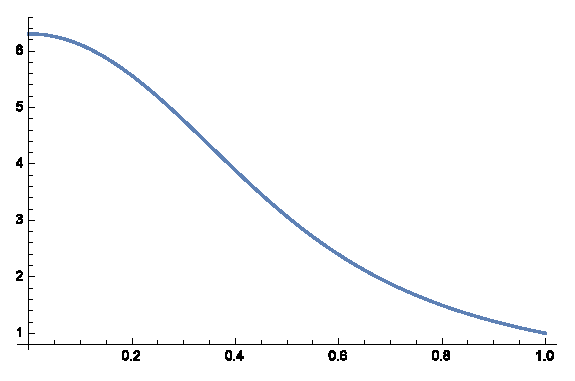
\includegraphics[width=3in]{ass3no4}
\end{figure}
\eenum





\enddocument} 